% Modelo de slides para projetos de disciplinas do Abel
\documentclass[10pt]{beamer}

\usetheme[progressbar=frametitle]{metropolis}
\usepackage{appendixnumberbeamer}
\usepackage[numbers,sort&compress]{natbib}
\bibliographystyle{plainnat}

\usepackage{booktabs}
\usepackage[scale=2]{ccicons}

\usepackage{xspace}
\newcommand{\themename}{\textbf{\textsc{metropolis}}\xspace}

\title{Analysis}
% \subtitle{Subtítulo}
% \date{\today}
\date{}
\author{Shuo Jia}
%\institute{UFPR - Disciplina - Semestre}
% \titlegraphic{\hfill\includegraphics[height=1.5cm]{logo.pdf}}

\begin{document}

\maketitle

%\begin{frame}{Table of contents}
%  \setbeamertemplate{section in toc}[sections numbered]
%  \tableofcontents[hideallsubsections]
%\end{frame}

%\section{Introduction}

\begin{frame}[fragile]{reference time}
Pre-trigger to all ADCs/TDCs in all detector Readout Controllers(ROCs)

Reference time is subtracted from detector signal

Analyzer considers first hit after cut to be a good hit

  
\end{frame}

\begin{frame}{}

\begin{minipage}{0.5\textwidth}
\begin{figure}[H]
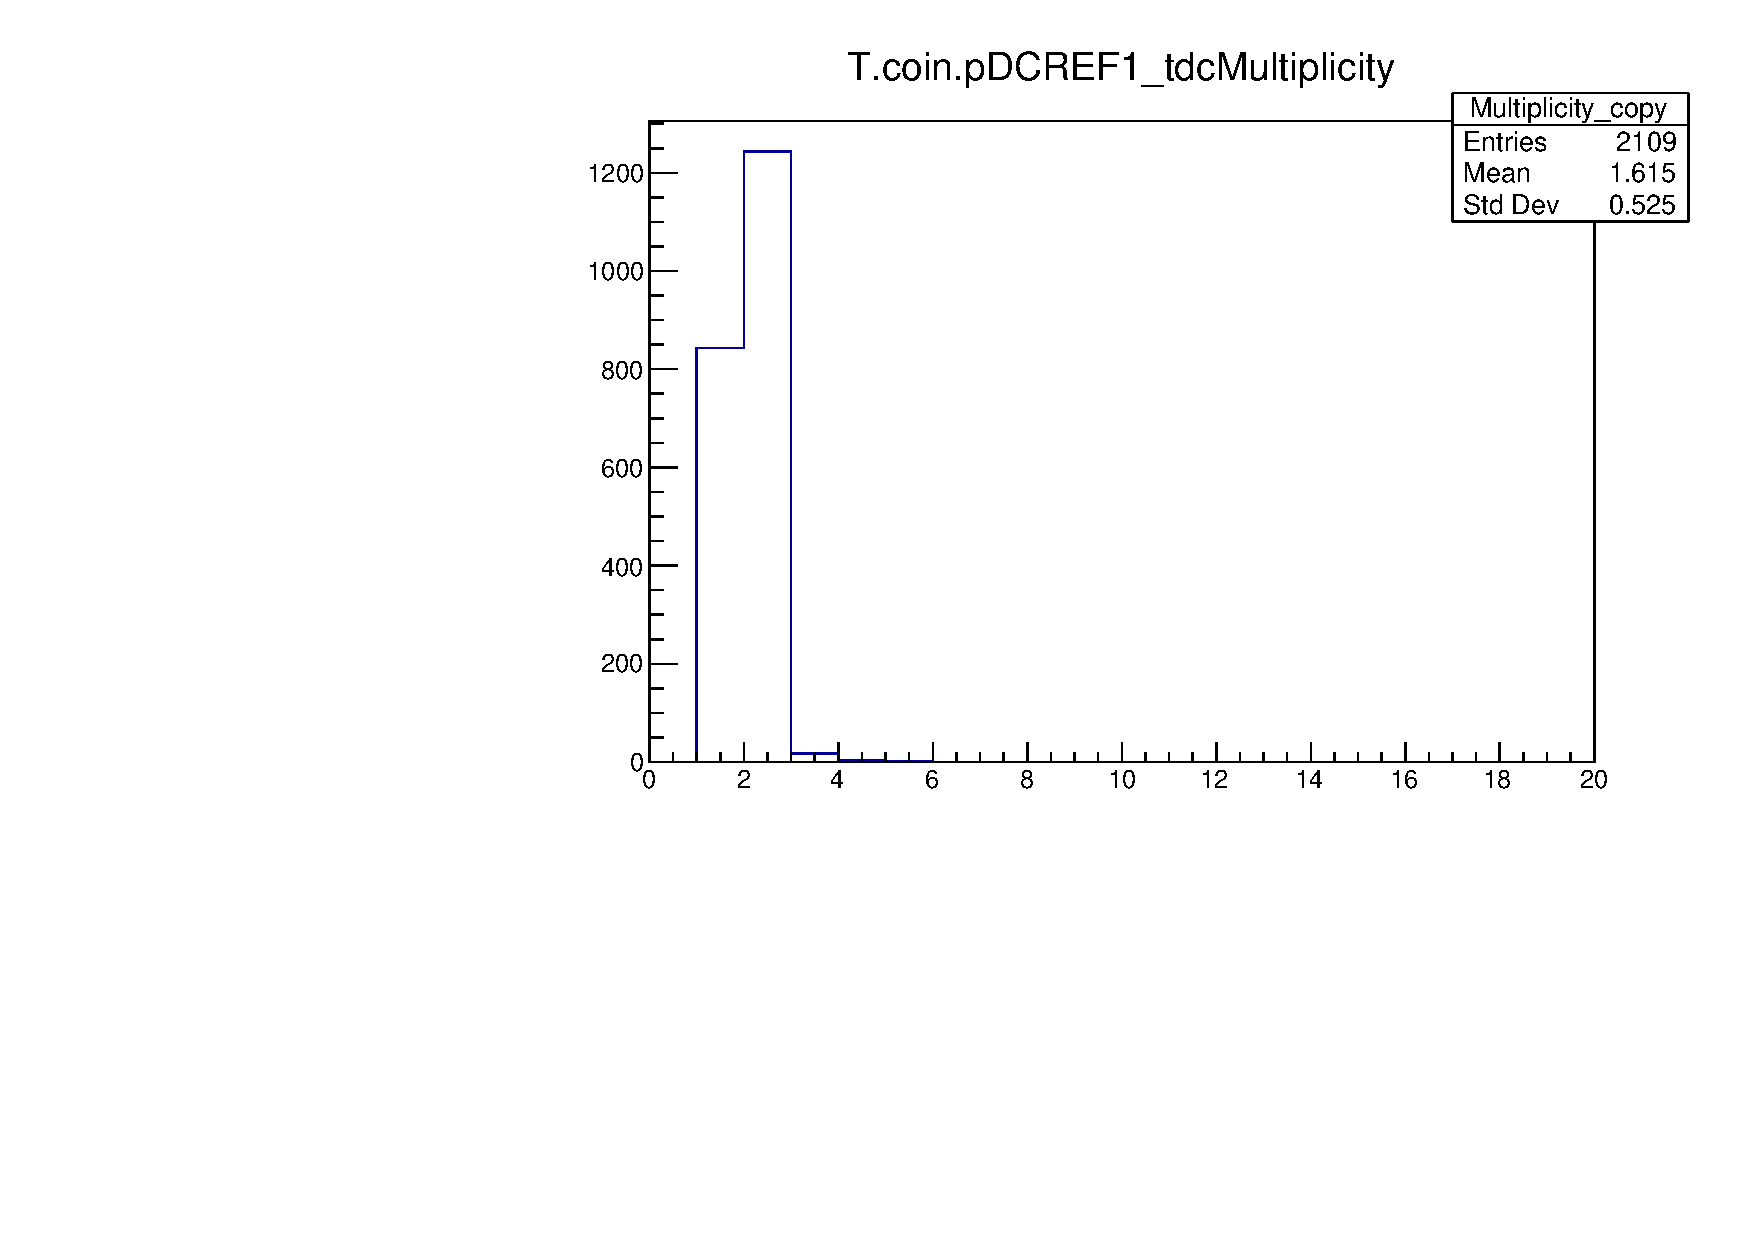
\includegraphics[width = \textwidth]{multiplicity.pdf}
\caption{\label{multiplicity} Multiplicity}
\end{figure}
\end{minipage} \hfill
\begin{minipage}{0.45\textwidth}
The multiplicity of a given variable refers to the total number of adc or tdc hits per event. 
\end{minipage}
   

\end{frame}{}

\begin{frame}{}
    \begin{figure}
    \centering
    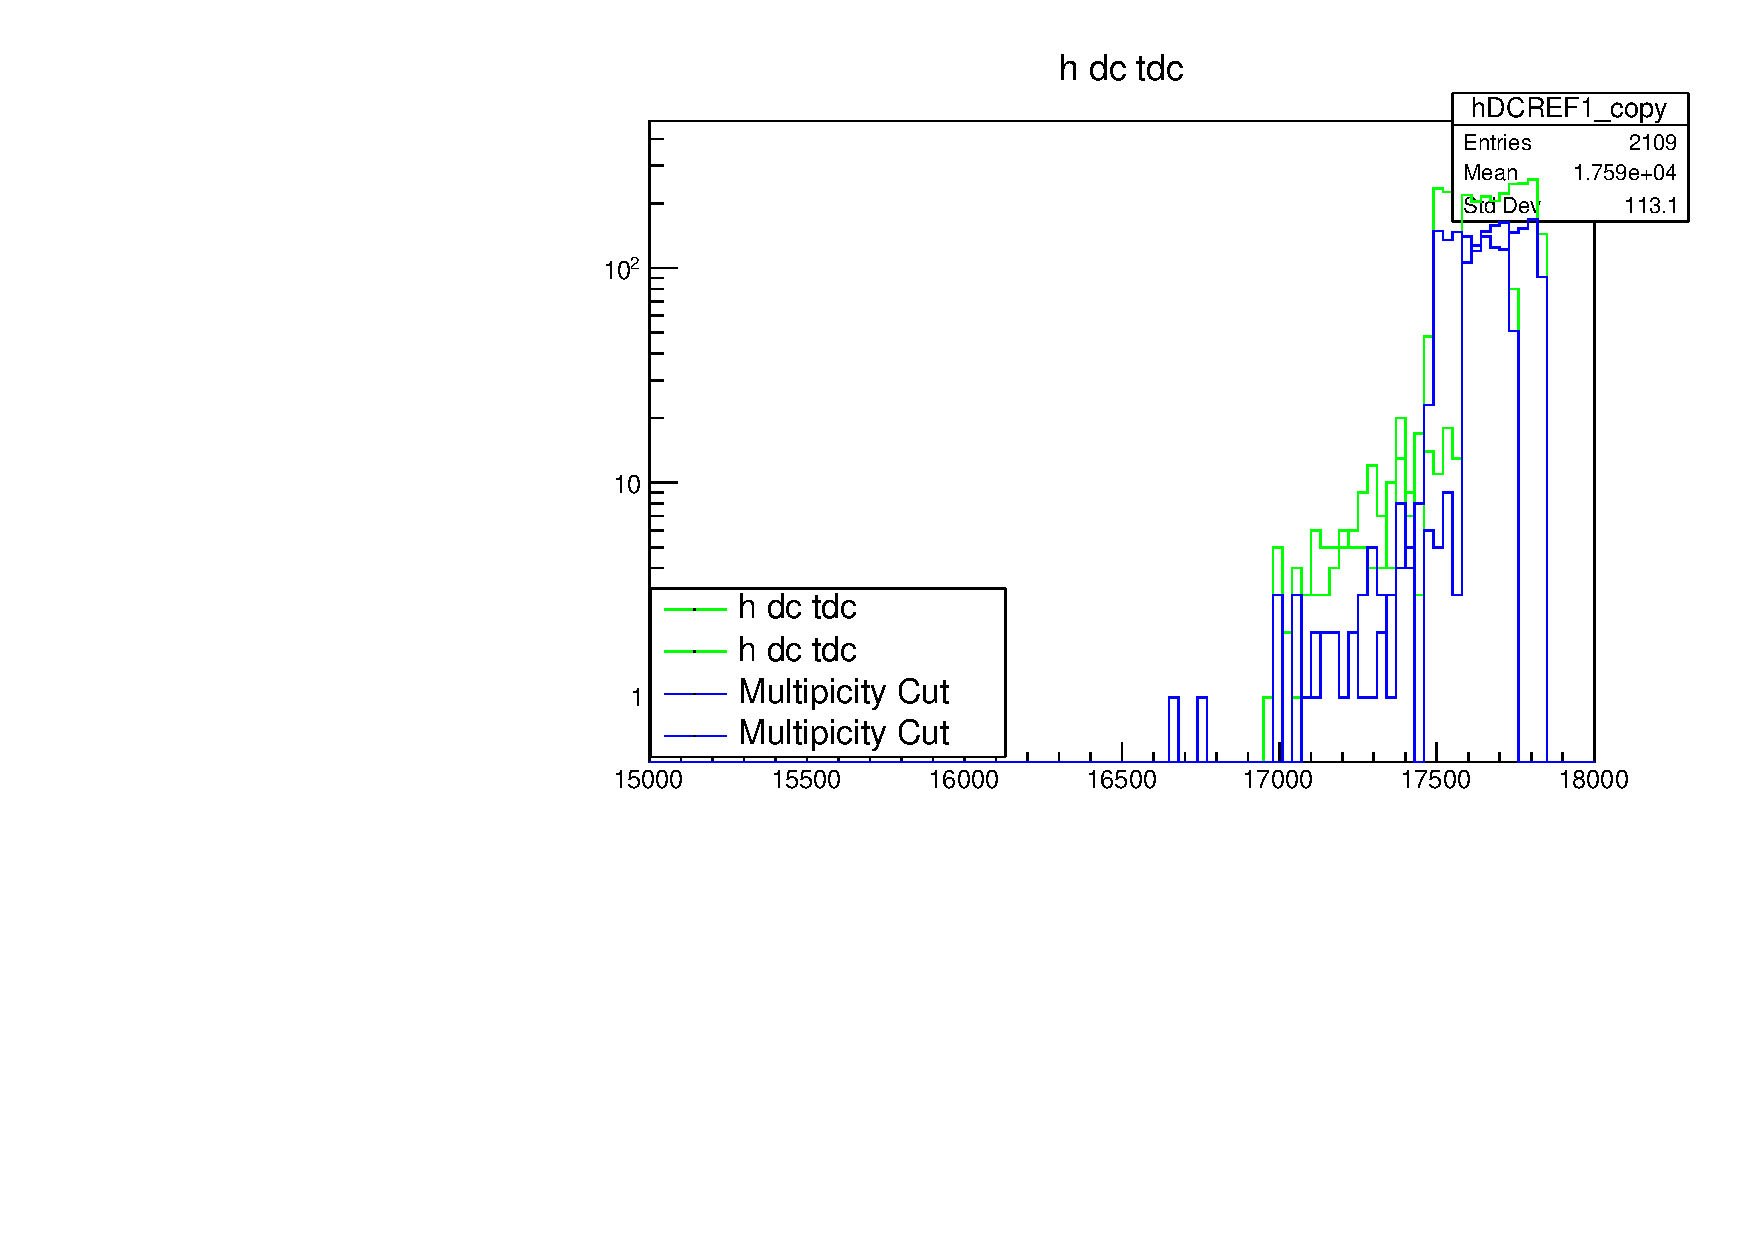
\includegraphics[width=\textwidth]{h_dc_tdc.pdf}
    \caption{HMS Drift Chamber TDC reference time cut}
    %\label{}
\end{figure}{}
\end{frame}{}

\begin{frame}{}
    \begin{figure}
    \centering
    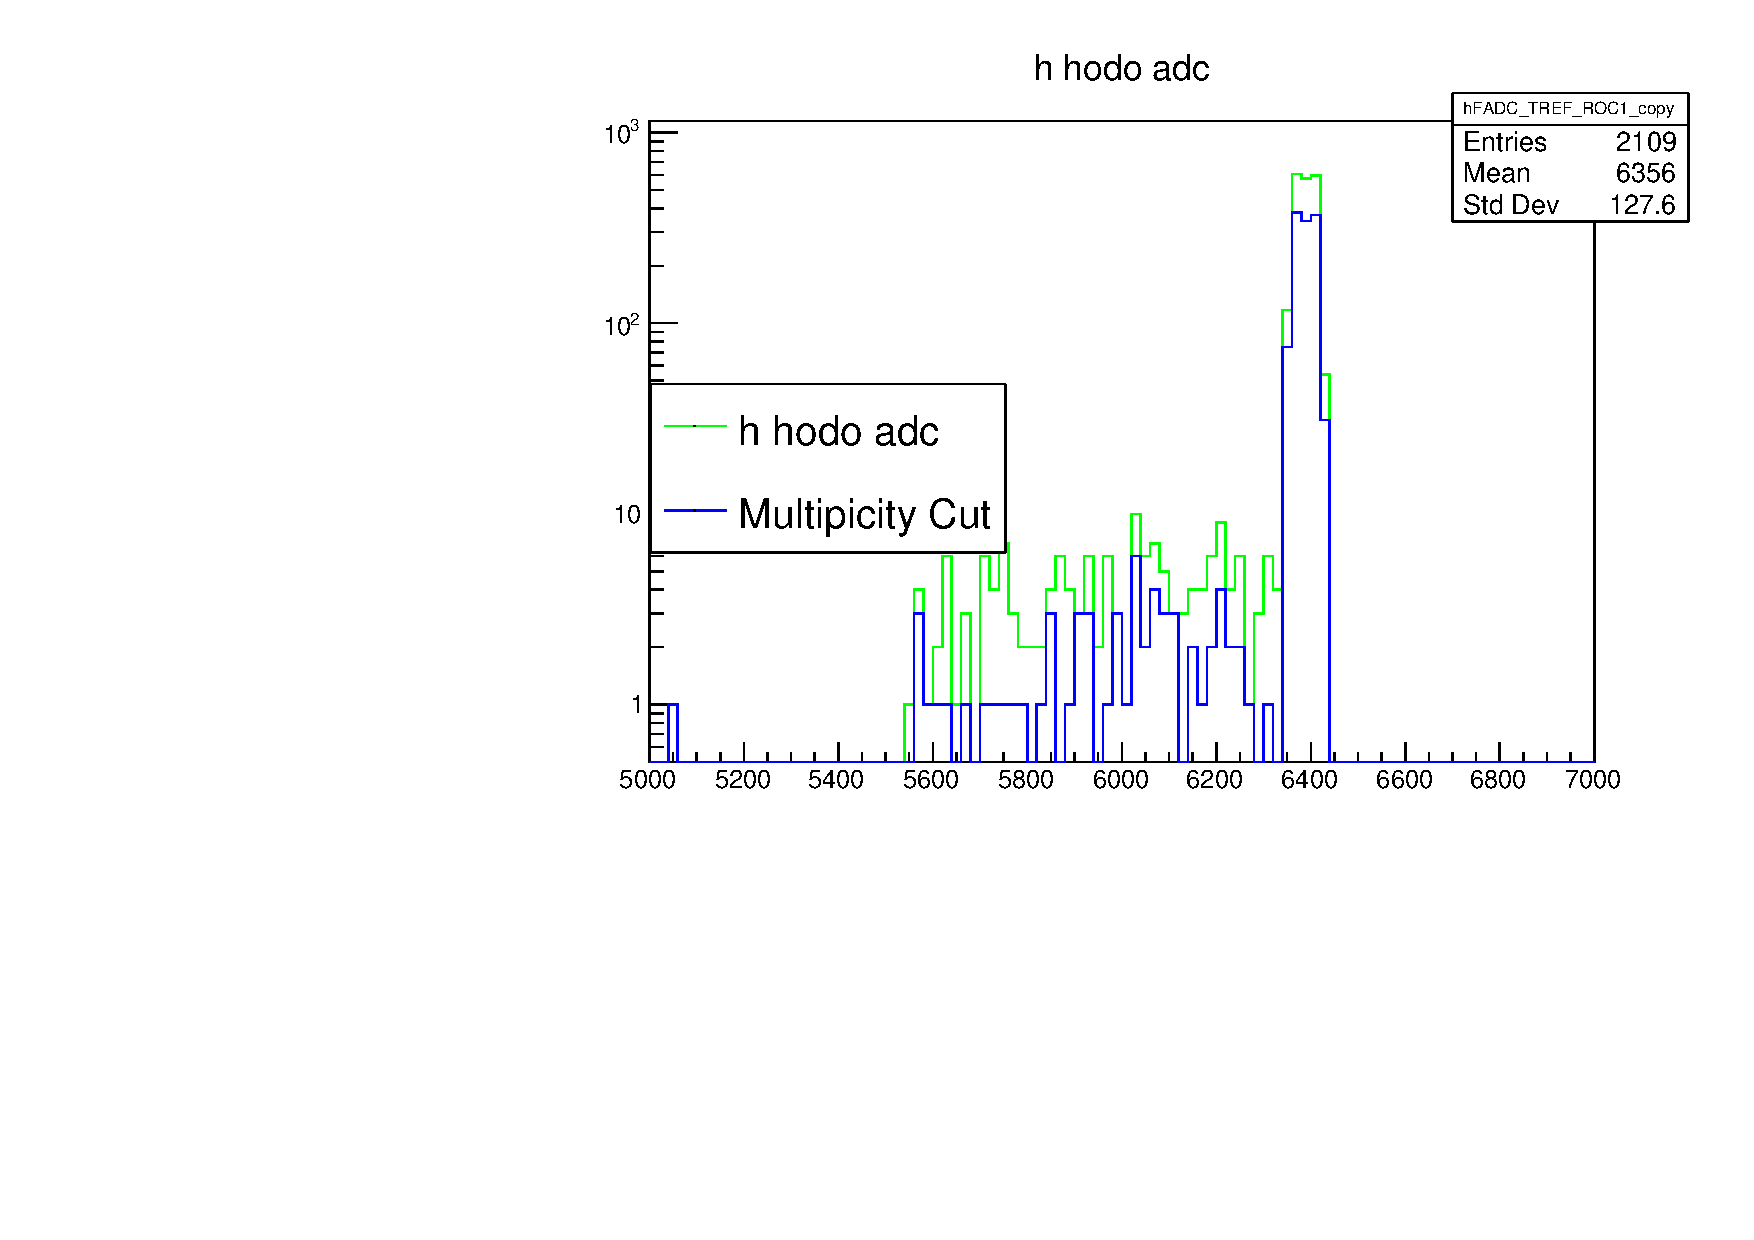
\includegraphics[width=\textwidth]{h_hodo_adc.pdf}
    \caption{HMS hodoscope ADC reference time cut}
    %\label{}
\end{figure}{}
\end{frame}{}

\begin{frame}{}
    \begin{figure}
    \centering
    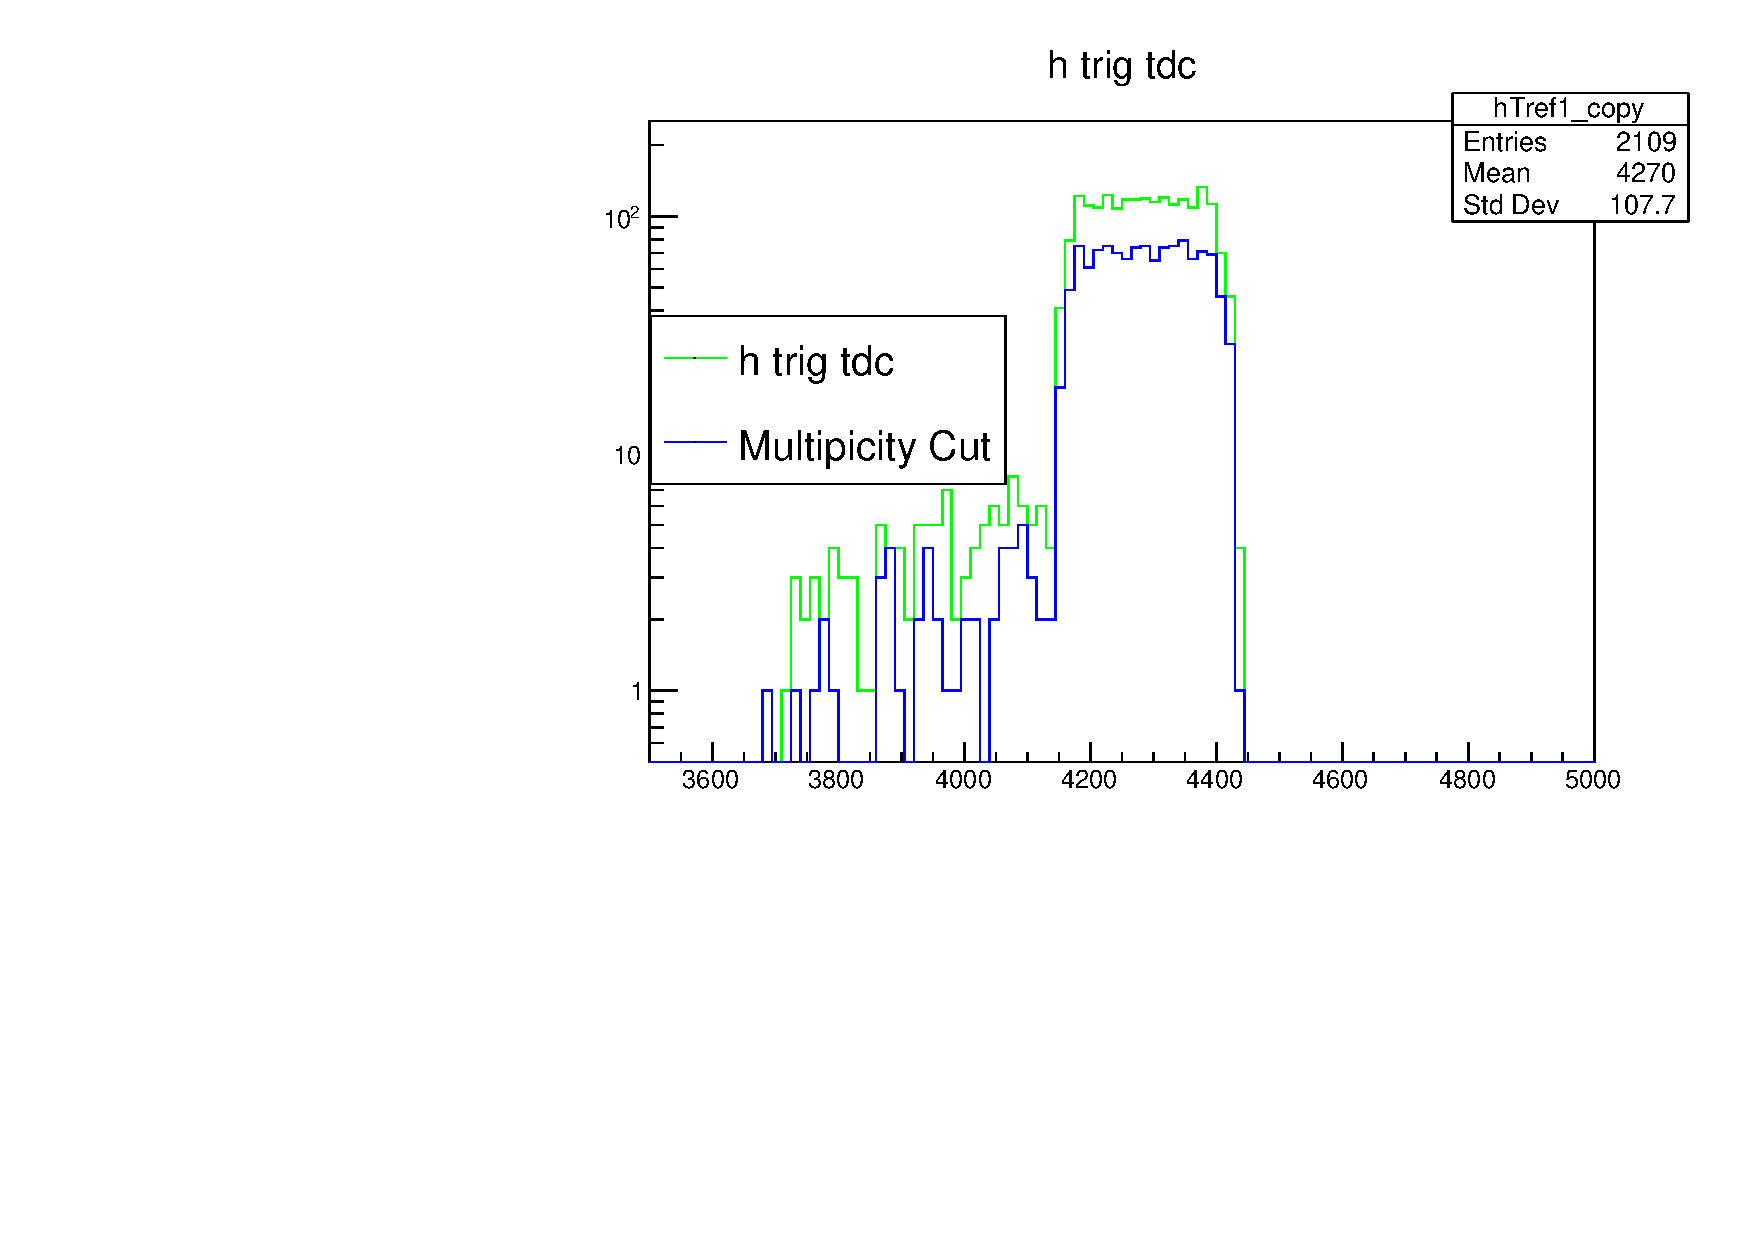
\includegraphics[width=\textwidth]{h_trig_tdc.pdf}
    \caption{HMS Trigger TDC reference time cut}
    %\label{}
\end{figure}{}
\end{frame}{}

\begin{frame}{}
    \begin{figure}
    \centering
    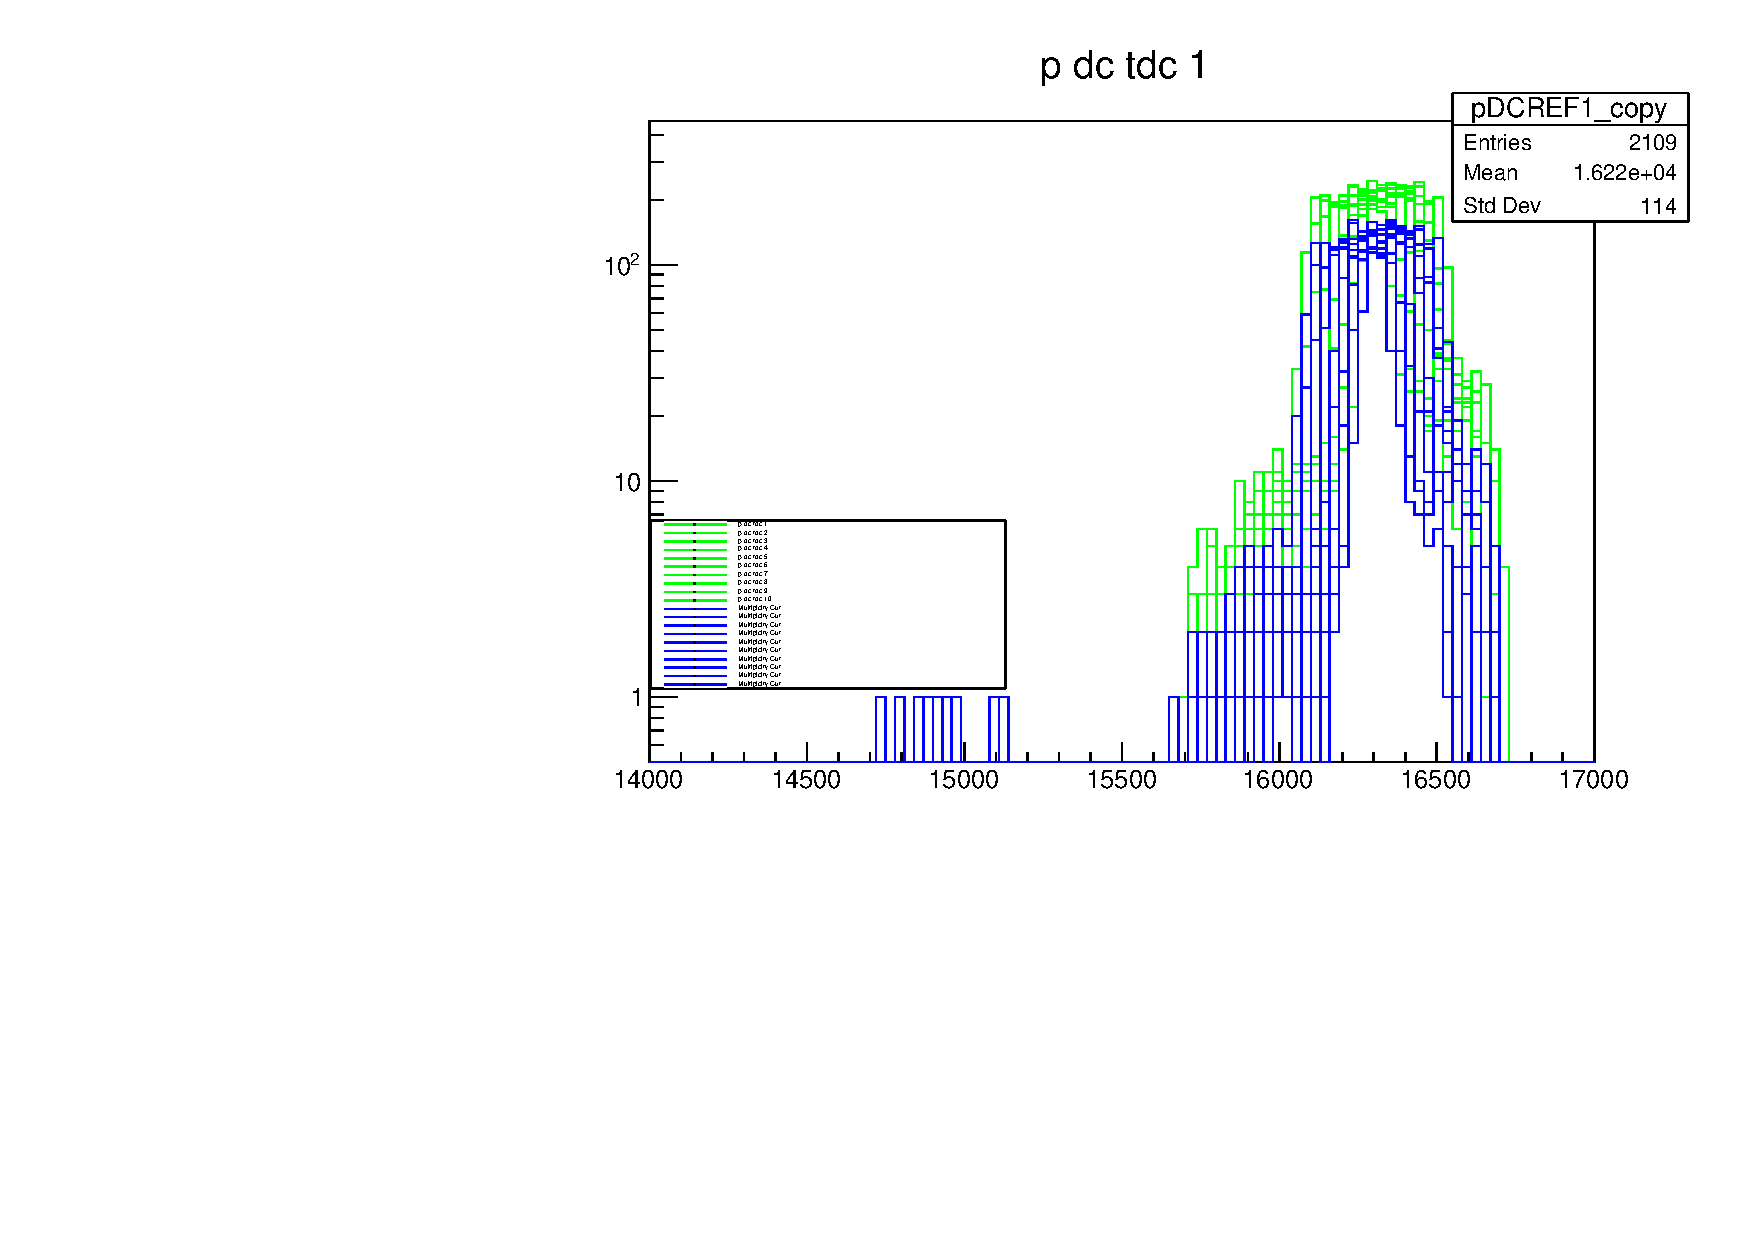
\includegraphics[width=\textwidth]{p_dc_tdc.pdf}
    \caption{SHMS Drift Chamber TDC reference time cut}
    %\label{}
\end{figure}{}
\end{frame}{}

\begin{frame}{}
    \begin{figure}
    \centering
    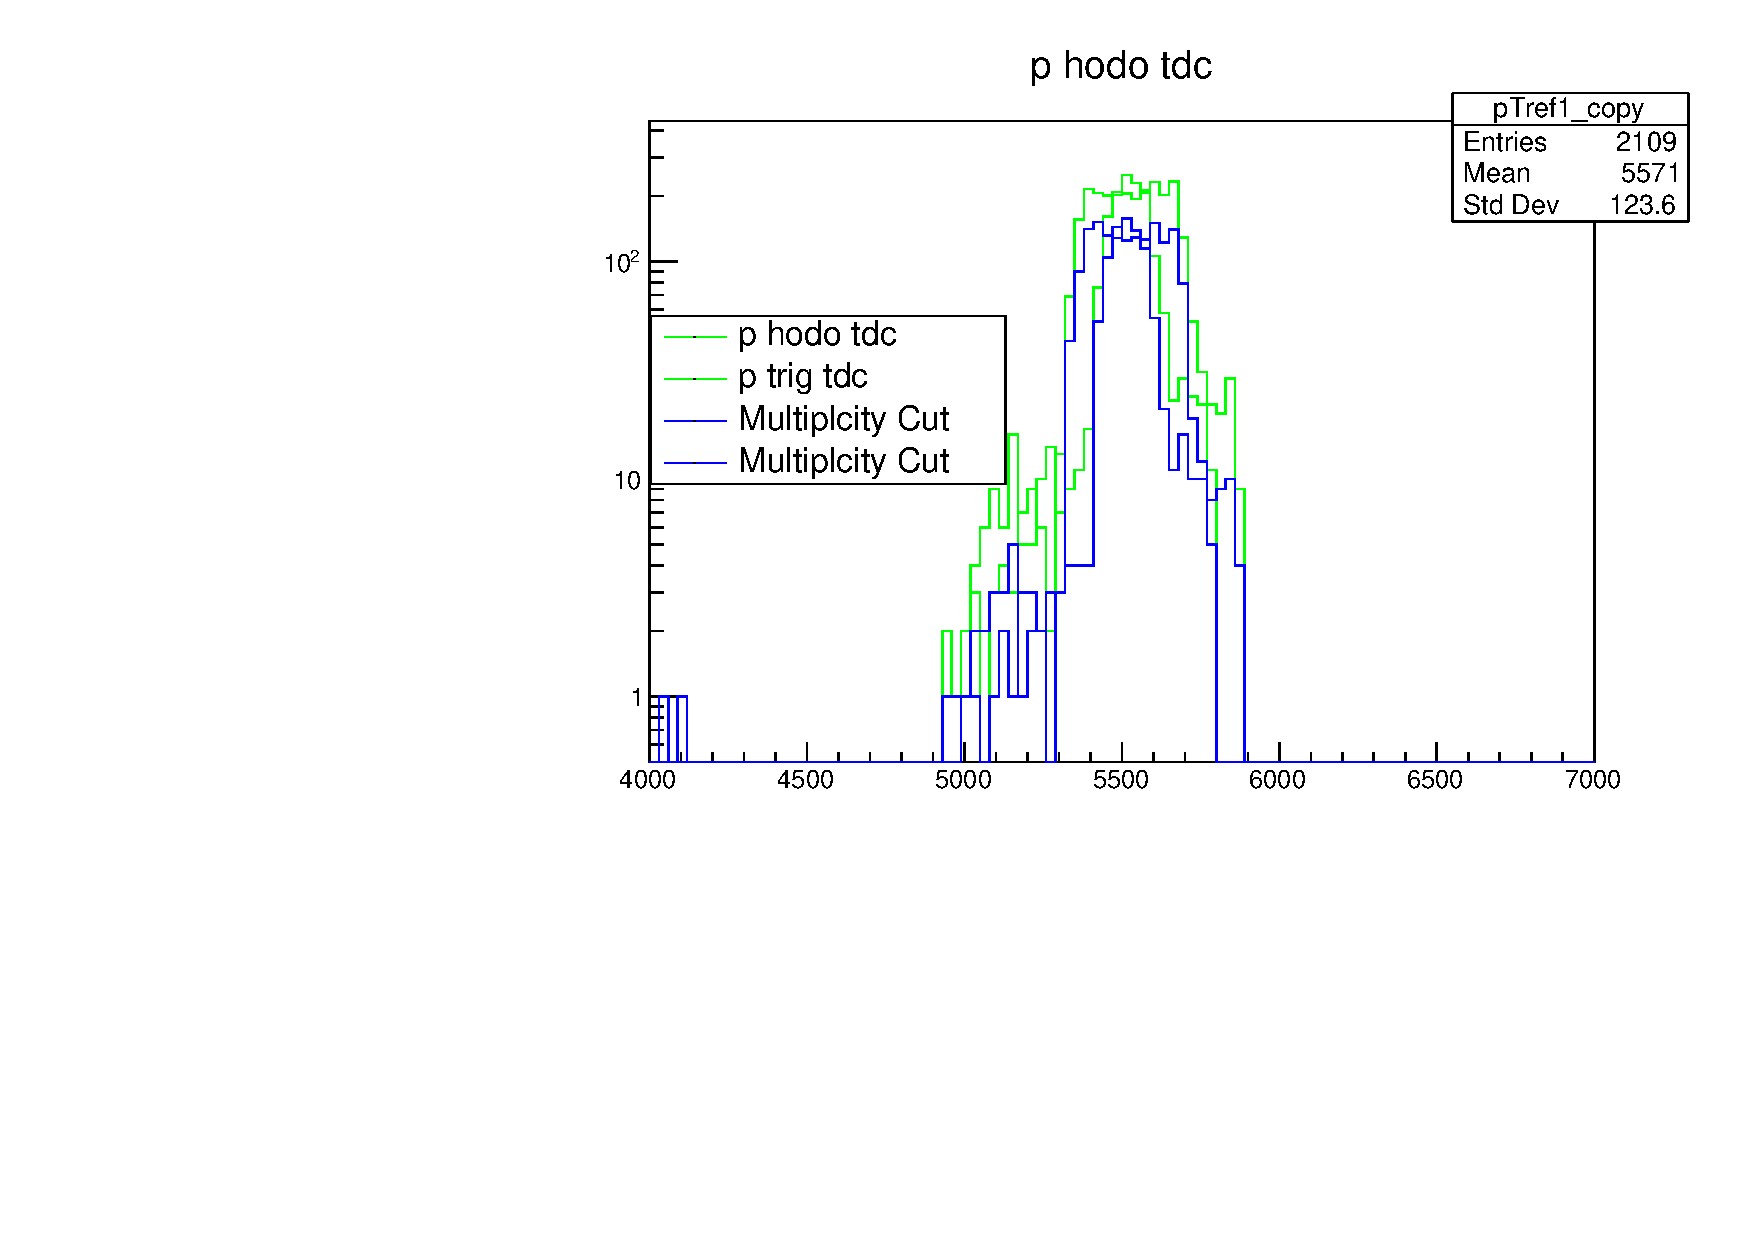
\includegraphics[width=\textwidth]{p_hodo_tdc.pdf}
    \caption{SHMS hodoscope TDC reference time cut}
    %\label{}
\end{figure}{}
\end{frame}{}

\begin{frame}{}
    \begin{figure}
    \centering
    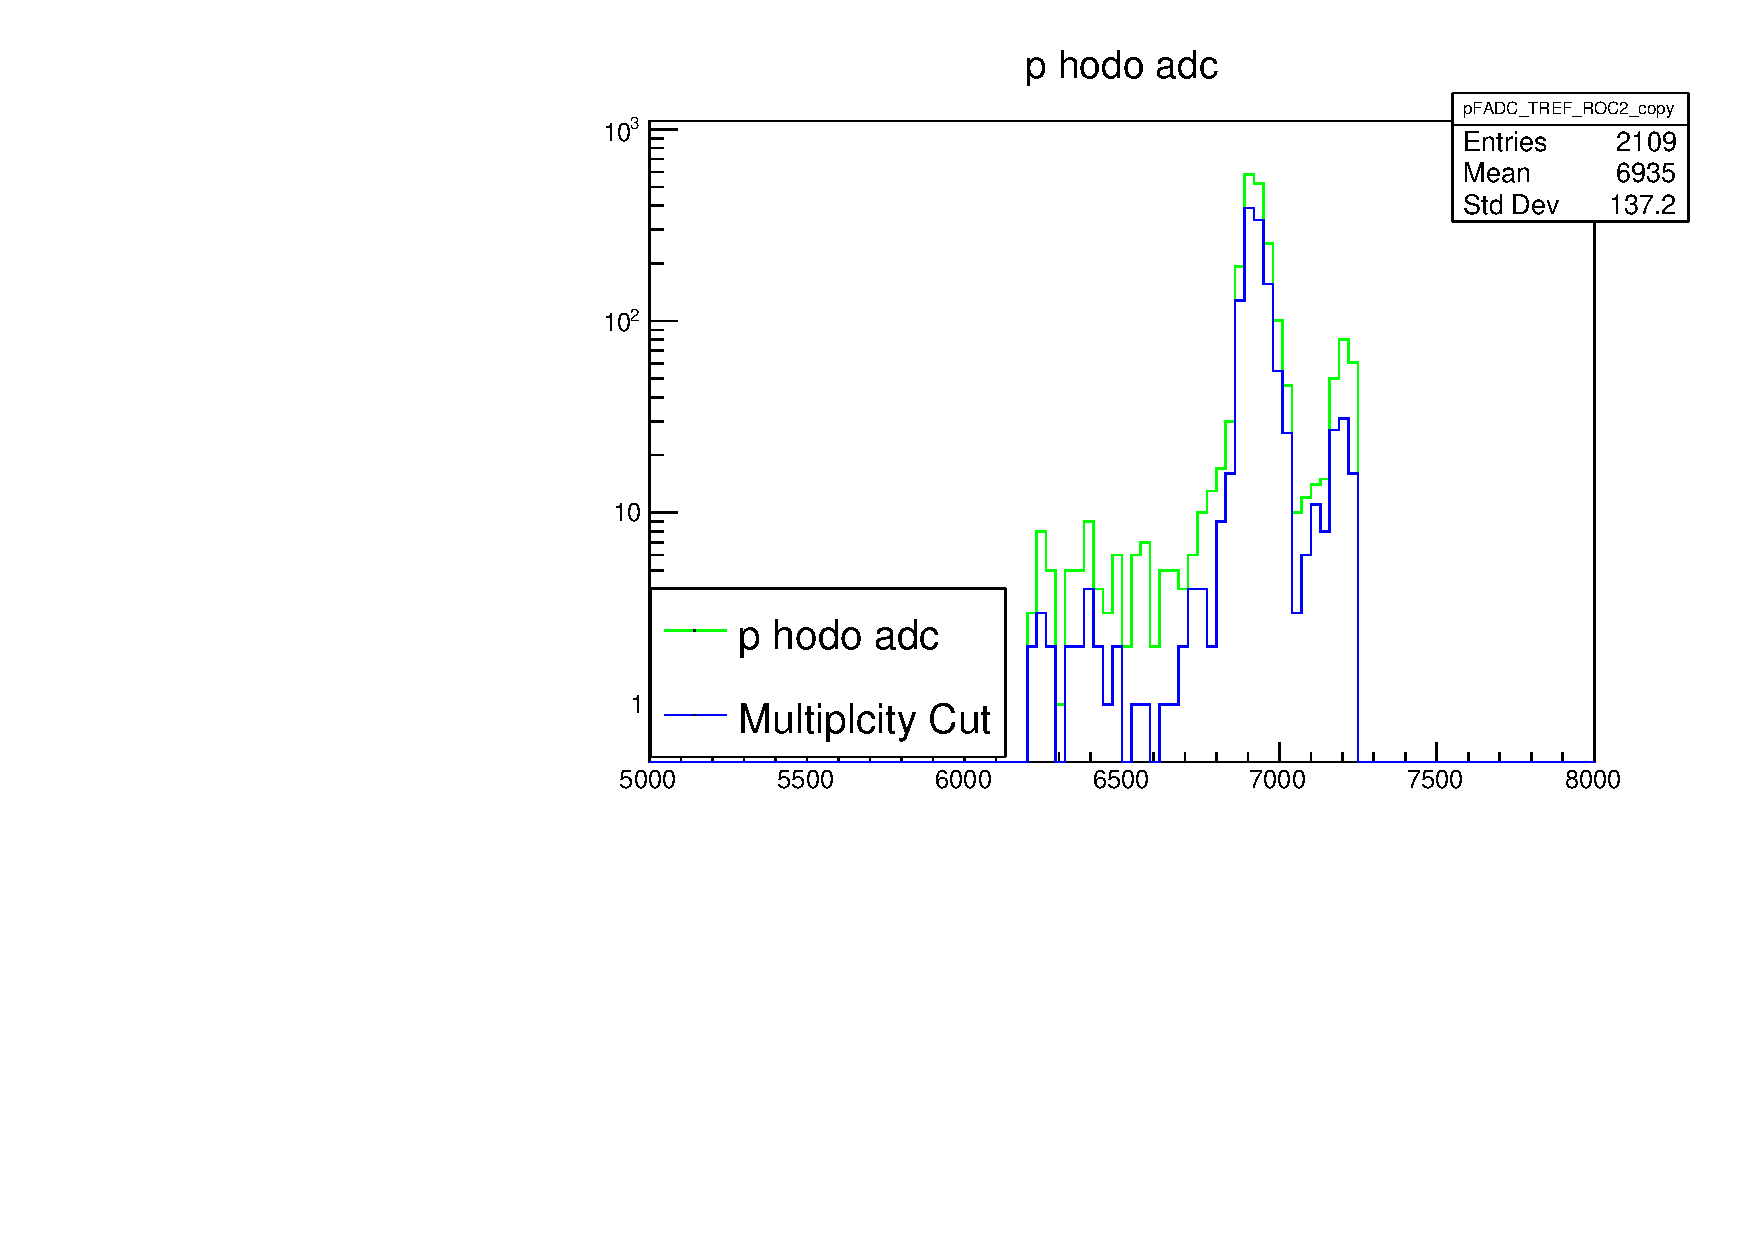
\includegraphics[width=\textwidth]{p_hodo_adc.pdf}
    \caption{SHMS hodoscope ADC reference time cut}
    %\label{}
\end{figure}{}
\end{frame}{}

\begin{frame}{}
    \begin{figure}
    \centering
    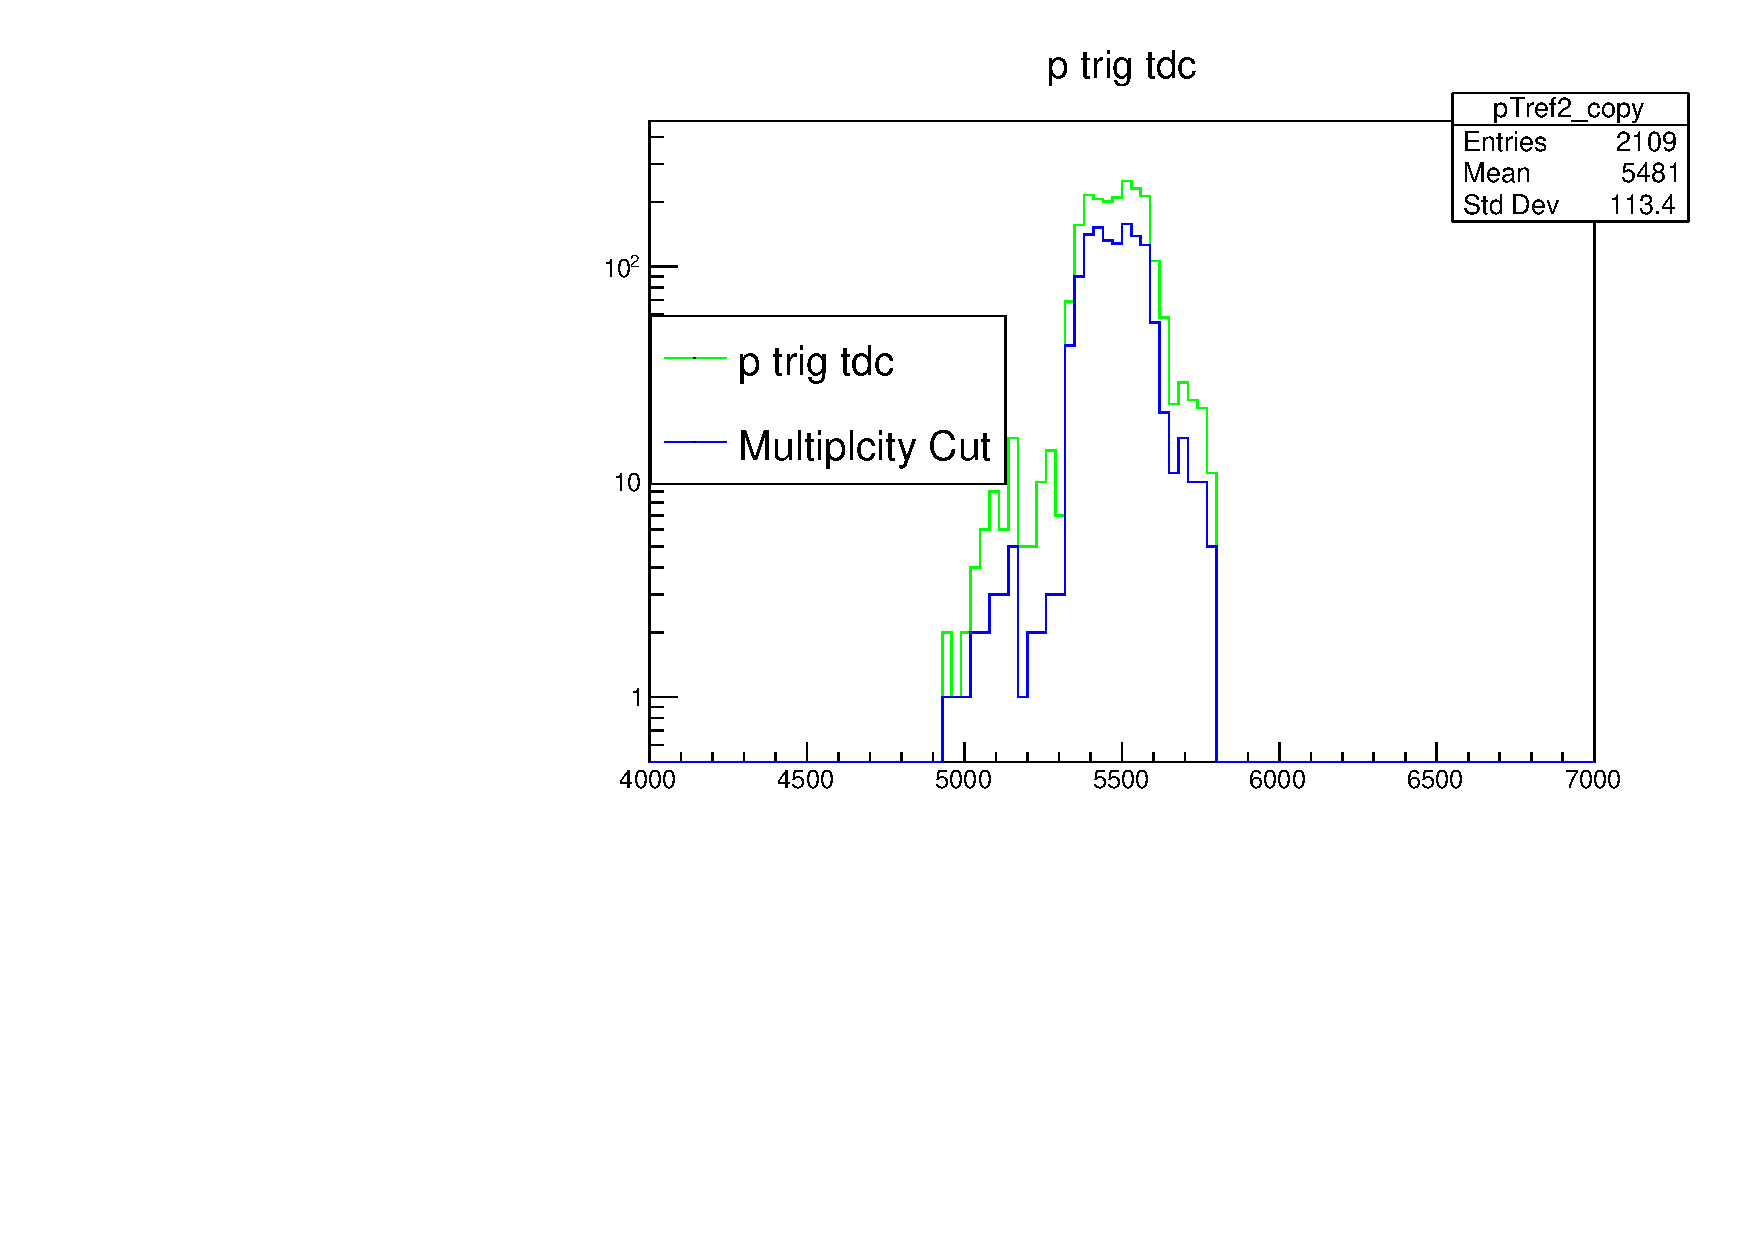
\includegraphics[width=\textwidth]{p_trig_tdc.pdf}
    \caption{SHMS trigger TDC reference time cut}
    %\label{}
\end{figure}{}
\end{frame}{}

\begin{frame}{}
  \begin{figure}[!tbp]
  \centering
  \begin{minipage}[b]{0.4\textwidth}
    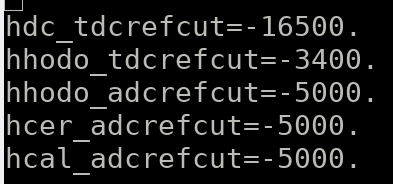
\includegraphics[width=\textwidth]{h_ref_cut.png}
    \caption{HMS refertime cut}
  \end{minipage}
  \hfill
  \begin{minipage}[b]{0.4\textwidth}
    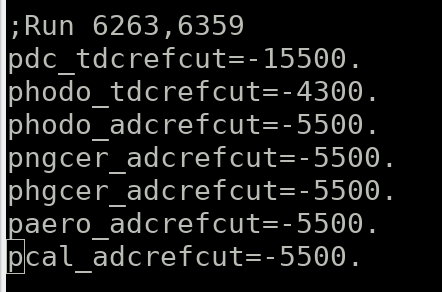
\includegraphics[width=\textwidth]{p_ref_cut.png}
    \caption{SHMS refertime cut}
  \end{minipage}
\end{figure}
\end{frame}{}

\begin{frame}{Detector time window cut}
    AdcTdcTime difference is defined as
    \begin{align}\label{CSV(X)}
    \begin{split}
             TdcTime[ipmt]-AdcPulseTime[ipmt] &= Hodo, \\
        HodoStartTime - AdcPulseTime[ipmt] &=CER, CAL, AERO
    \end{split}
\end{align}
    HodoStartTime is the Hodoscope time projected at the focal plane, and the TdcTime, AdcPulseTime is the
detector (TDC,ADC) pulse time for a given PMT in that detector.

Due to the finite detector resolutions, event has
a finite width and gaussian in shape time

Did we finish this? 
    \end{frame}{}
\end{document}
